\section{Servlet}

% hier bitte die Grafik der Servlets
\begin{figure}[h]
\centering
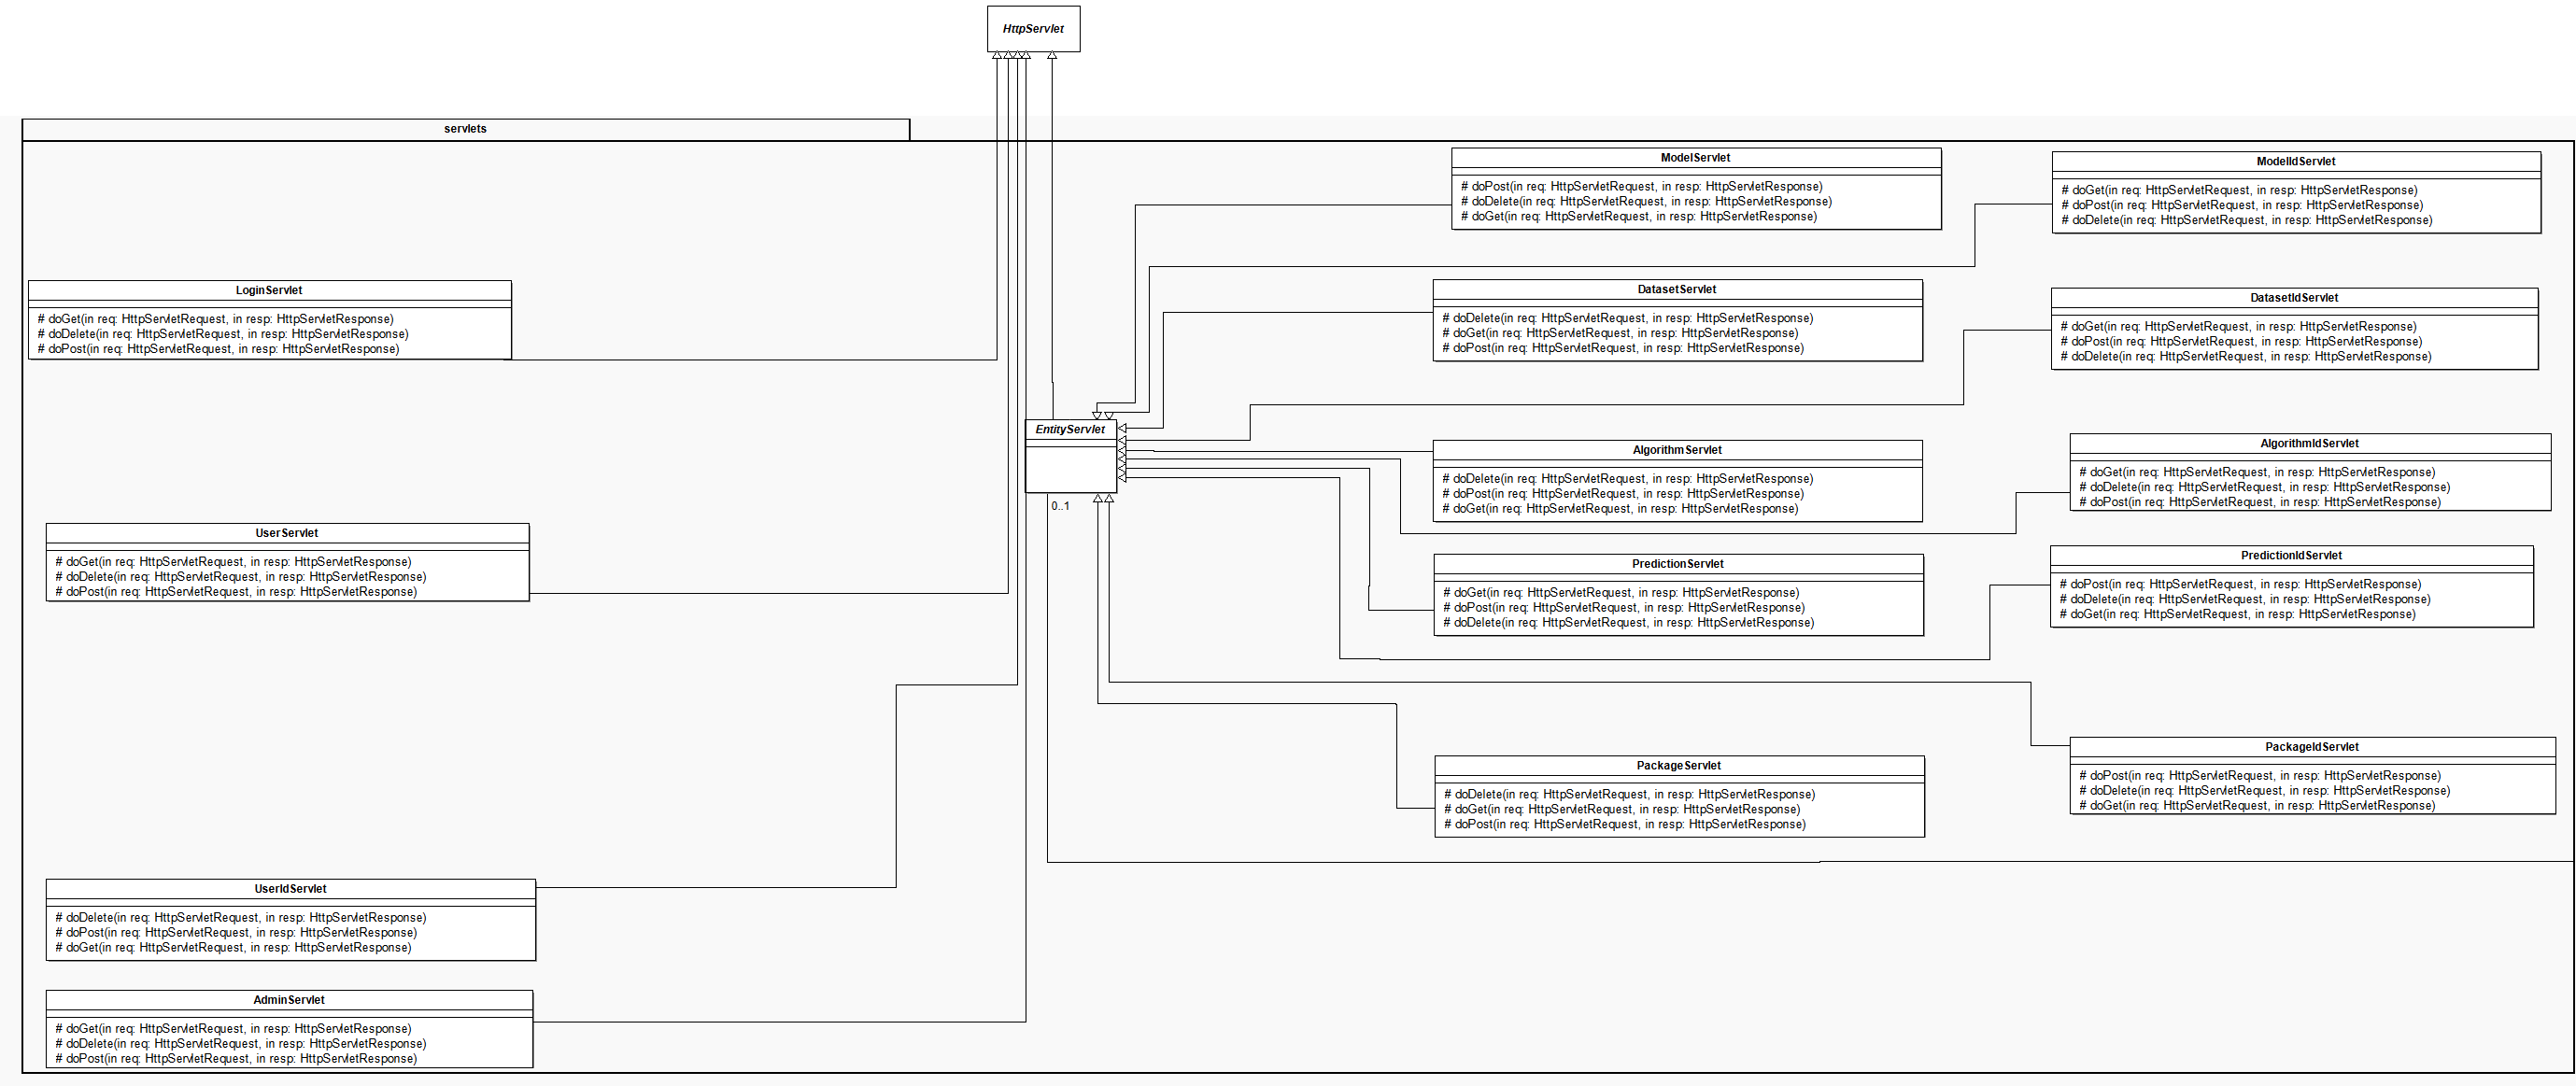
\includegraphics[width=0.9\linewidth]{Grafik/Klassendiagramme/Servlet.png}
\caption{Übersicht aller Servlets}
\end{figure}


Der Server implementiert verschiedene Servlets, die die Anfragen eines Clients entgegennehmen und beantworten. Hierzu werden die Anfragen des Nutzer ausgewertet und in der Klassenhierarchie an die zuständigen Instanzen weitergeleitet. Zu jedem REST Endpoint den das System bereitstellt existiert ein entsprechendes Servlet, welches von dem javax.servlet.http.HttpServlet abgeleitet ist. Durch diese Implementierung können leicht weitere Endpoints hinzugefügt werden, falls die nötig sein sollte. Jede Subklasse überschreit hierbei die ''doGet'' und ''doPost'' Methode, um die gewünschte Operation entsprechend der Art der Anfrage auszuführen. Hierzu kommuniziert die Servlet Klasse mit einer Subklasse des EntityControllers, der nach dem Model-View-Controller Pattern mit dem EntityModel und dem EntityView interagiert. Der EntityView realisiert hierbei den dynamischen Web-Inhalt, der dem Benutzer auf Anfrage angezeigt wird. Für jede verfügbare Ansicht existieren entsprechende Subklassen dieser drei MVC Klassen, die den jeweils benötigten Inhalt bereitstellen. 


\subsection{Abstrakte MVC-Klassen}

\begin{figure}[h]
\centering
\includegraphics[width=0.4\linewidth]{Grafik/Klassendiagramme/Entity_mvc.png}
\caption{Entity MVC}
\end{figure}
